\documentclass[12pt,a4paper]{article}
\usepackage[latin1]{inputenc}
\usepackage[spanish]{babel}
\usepackage{graphicx}
\usepackage[left=1.3cm,right=1.3cm,top=1.8cm,bottom=4cm]{geometry}
\usepackage{lastpage}
\usepackage{marginnote}
\usepackage{multirow}
\usepackage{wallpaper}
\usepackage{fancyhdr}
\setlength{\headheight}{87pt} 
\pagestyle{fancy}\fancyhf{}
\renewcommand{\headrulewidth}{0pt} 
\setlength{\parindent}{0cm}
\newcommand{\tab}{\hspace*{2em}}
\newcommand\BackgroundStructure{
\setlength{\unitlength}{1mm}
\setlength\fboxsep{0mm}
\setlength\fboxrule{0.5mm}
\put(10, 10){\fcolorbox{black}{white!10}{\framebox(192,247){}}}
\put(10, 262){\fcolorbox{black}{white!10}{\framebox(192, 31){}}}
}

%-------------------------ENCABEZADO---------------
\fancyhead[L]{\begin{tabular}{l r | l r}	
\textbf{Proyecto} & 1 & \textbf{Página} & \thepage/\pageref{LastPage} \\
\textbf{Trabajo} & Desarrollo de un controlador & \textbf{Actualizado en:} & 27/08/2016 \\
\textbf{} &  VGA & \textbf{Revisado en:} & 07/04/2016 \\
\textbf{Grupo} & 1 & \textbf{Diseñadores} & Keylor Mena Venegas \\
\textbf{Revisado por:} & Alfonso Chacón Rodríguez & \textbf{ } & Luis Leon Vega \\
\textbf{} & & \textbf{ } & Luis Merayo Gatica
\end{tabular}}

\begin{document}
\AddToShipoutPicture{\BackgroundStructure}

\section{Resumen} 
Muchos de los monitores que se emplean, actualmente, en computadoras personales emplean el protocolo de comunicación de video VGA (Video Graphics Array). Este protocolo fue diseñado para controlar monitores basados en la tecnología de tubos al vacío, específicamente, el tubo de rayos catódicos (CRT).\\[2ex]
El funcionamiento de estos monitores estaba basado en los televisores de esta misma tecnología, donde empleaban cañones de color controlados por los cátodos y dirigían el haz de electrones mediante electromagnetismo, logrando barrer la pantalla de fósforo que se ilumina gracias al choque de los electrones contra el material. \\[2ex]
No obstante, el protocolo continúa utilizándose en la actualidad, a pesar de que la tecnología CRT ha quedado en obscolescencia. Para este proyecto, se realizará un controlador de un monitor LCD que emplee el protocolo VGA, esto, empleando una FPGA Nexys 3 para poder implementar la lógica que se diseñará para construir el controlador y, de esta forma, acelerar el proceso de prototipado del diseño. \\ [2ex]
Finalmente, este documento contendrá el proceso de diseño del controlador, la comprobación del diseño mediante simulación y los resultados experimentales producto del prototipado y la implementación en la FPGA Nexys 3.

\section{Introducción} 
El controlador VGA a desarrollar en este proyecto contiene señales de sincronía vertical y horizontal que permiten barrer la pantalla de forma completa y, además, se requiere generar señales analógicas para modificar los tonos de color. En total, se deben diseñar etapas para poder generar la imagen, cambiar los colores y sincronizar la señal del monitor para que la tarea pueda realizarse de forma exitosa. \\[2ex]
Para la implementación se tomará en cuenta la placa de desarrollo Nexys 3 de Digilent, que posee una FPGA Spartan-6 de Xilinx y posee un convertidor de digital a analógico en la salida de los colores hacia el monitor que permite generar hasta 256 colores distintos (combinaciones de 3 tonos de rojo y verde y 2 tonos de color azul). Asimismo, la velocidad del reloj de este dispositivo es de 100 MHz, que equivale a 4 veces más, la frecuencia requerida para el proyecto, de acuerdo con Pong Chu [1]. \\[2ex]
Por otro lado, otras de las conveniencias para usar esta placa de desarrollo de Digilent es la posibilidad de desarrollar su descripción de hardware en el entorno de Xilinx ISE, que permite controlar la descripción en lenguajes HDL en cuanto a los recursos disponibles de la Spartan-6. Esto facilita el manejo de la implementación y brinda la posibilidad de emplear una basta cantidad de instrucciones embebidas al IDE (Entorno de desarrollo). \\[2ex]
Para concluir este apartado, se empleará la técnica de diseño Top-Down para poder crear un diseño de forma eficiente y, así, finalizar de acuerdo con el cronograma dispuesto como parte del plan de proyecto.

\section{Objetivos}
\begin{itemize}
    \item Proponer un diseño a nivel de bloques de un controlador VGA que sea capaz de desplegar caracteres o símbolos en 8 colores distintos.
    \item Emplear las técnicas de diseño Top-Down.
    \item Desarrollar el código en Verilog, verificarlo a nivel de simulación de post-síntesis y a una velocidad de reloj de al menos 100 MHz.
    \item Comprobar el funcionamiento mediante la implementación en una FPGA Nexys.
\end{itemize}

\section{Descripción del sistema}
El circuito controlador se ha definido en cuatro bloques principales, encargados de generar el barrido, los datos y la sincronía requerida para el funcionamiento del monitor mediante el protocolo VGA. A nivel general, el bloque de contadores son los que llevan el control del circuito en todo momento, permitiendo generar señales de sincronía y movilizar la memoria para poder decodificar los datos de una memoria en forma de matriz. Esta memoria alimenta el circuito de control de control para poder generar las señales de color. En la Figura \ref{fig:generalSys}.

\begin{figure}[hbtp]
	\centering
	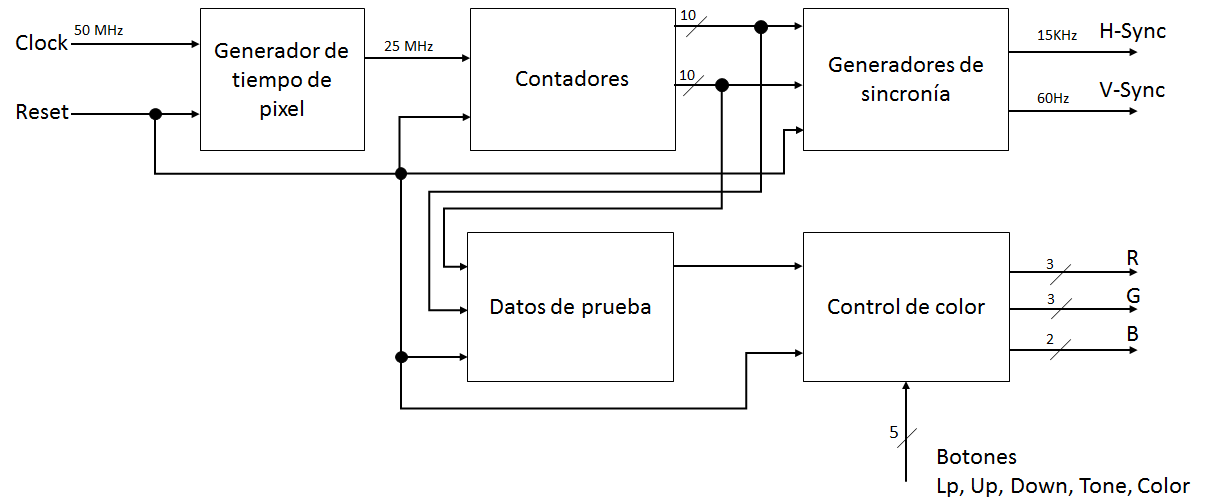
\includegraphics[width=18cm]{Img/diagramaIntro.png}
	\caption{Diagrama de bloques general del controlador VGA}
	\label{fig:generalSys}
\end{figure}

\subsection{Diseño Top-Down del circuito}
\subsubsection{Diagrama de primer nivel}  \label{sec:VGA_pn}
Previo a comenzar el diseño, se han establecido las entradas y salidas del circuito para poder determinar las necesidades que deben ser cubiertas. El diagrama de entradas y salidas se muestra en la Figura \ref{fig:PrimerNivel}. \\[2ex]
En cuanto a las entradas, se encuentran las principales para el funcionamiento del circuito, las cuales son el reloj (Clock) y el reinicio (Reset). Estos permiten a los circuitos secuenciales trabajar de forma adecuada. Por otro lado, se encuentran los selectores de tono (Tone) y color de letra-pantalla (LP). En el caso del selector de tono, este permite modificar la tonalidad del color de la pantalla o de las letras; si este selector no está habilitado, el color primario \textquotedblleft RGB \textquotedblright será cambiado. En el segundo caso, del selector color de letra-pantalla, este permite distinguir si se quiere cambiar el color del letra o de la pantalla. Finalmente, los botones de \textquotedblleft Up \textquotedblright y \textquotedblleft Down \textquotedblright, que permiten alterar los valores en función de la configuración en los selectores, anteriormente, mencionados. \\[2ex]
Para las salidas, se tienen las esenciales para el funcionamiento correcto del monitor mediante el protocolo VGA, las cuales son las señales de sincronía vertical y horizontal; \textquotedblleft V-Sync \textquotedblright y \textquotedblleft H-Sync \textquotedblright de forma respectiva. Y, se tiene además, las señales de datos analógicos de color; \textquotedblleft R \textquotedblright, \textquotedblleft G \textquotedblright y \textquotedblleft B \textquotedblright, que corresponden al color rojo, verde y azul, respectivamente.

\begin{figure}[htbp]
  \centering
    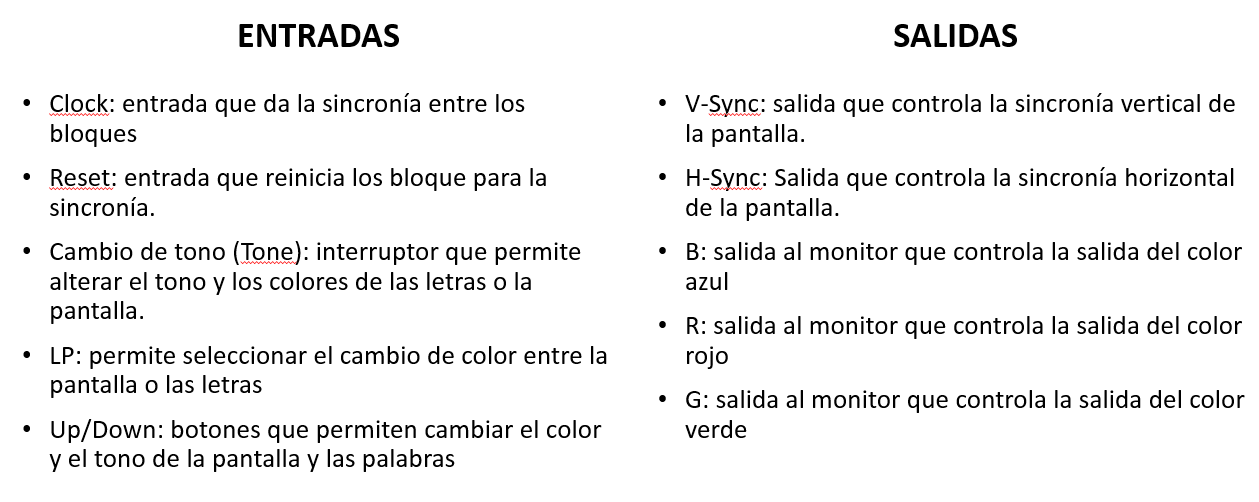
\includegraphics[width=18cm]{Img/PrimerNivel.png}
  \caption{Diagrama de primer nivel del VGA.}
  \label{fig:PrimerNivel}
\end{figure}

\subsubsection{Diagrama de segundo nivel} \label{sec:VGA_sn}
Un acercamiento a más profundo al diseño del proyecto se brinda en el segundo nivel de diseño mostrado en la Figura \ref{fig:SegundoNivel}. Este diagrama se acerca más a la realidad del circuito necesitado para conformar el controlador VGA. Al igual como se describió en la descripción del sistema, el diseño contempla a los contadoradores fundamentales para controlar el circuito en su totalidad. 

\begin{figure}[htbp]
  \centering
    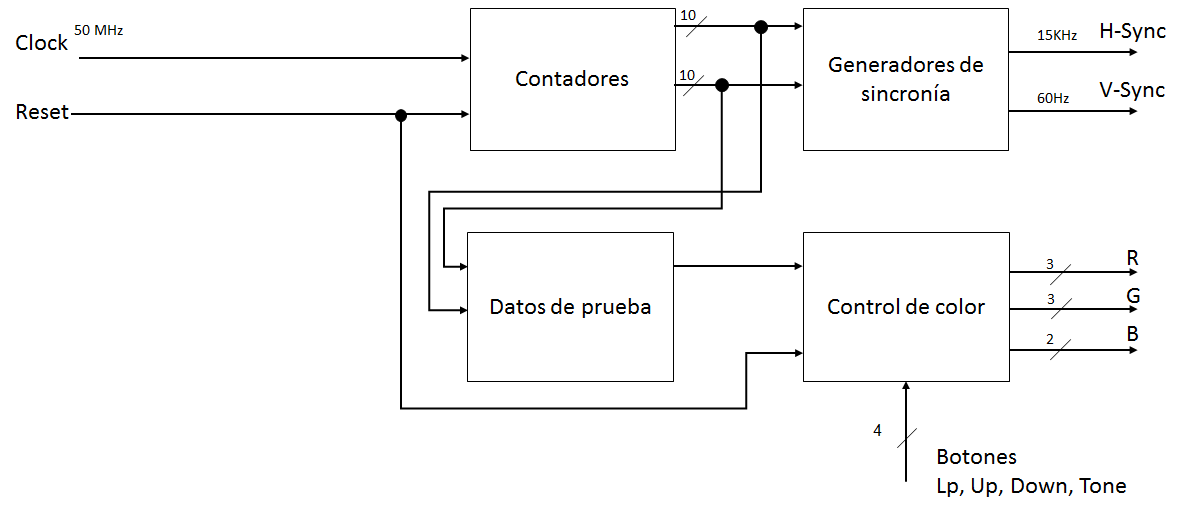
\includegraphics[height=6cm, width=16cm]{Img/SegundoNivel.png}
  \caption[2doNivel]{Diagrama de segundo nivel del VGA.}
  \label{fig:SegundoNivel}
\end{figure}

Los contadores, en este caso, son los encargados de llevar el conteo de las filas y columnas que se desplegarán en la pantalla del monitor conectado al circuito. Estos contadores suministrarán bus hacia los \textquotedblleft Generadores de Sincronía \textquotedblright para poder establecer una correcta conexión del monitor con el controlador. Asimismo, se alimenta el bloque de \textquotedblleft Datos de prueba \textquotedblright, que permitirá señalar a la etapa siguiente, \textquotedblleft Control de color \textquotedblright, cuando debe escribir la letra, poner fondo de pantalla y apagar la señal para generar los \textquotedblleft blank \textquotedblright. \\[2ex]
El \textquotedblleft Control de color \textquotedblright permite establecer el color que se pone en el fondo de la pantalla y a las letras. Esto de acuerdo con lo seleccionado por el usuario mediante el uso de los selectores de tono (Tone), de letra-pantalla (LP) y los botones Up/Down. Además, permite disernir cuando se debe colocar la pantalla en \textquotedblleft blank \textquotedblright durante los fragmentos de la señal de sincronía que no son escribibles.

\subsubsection{Diagrama de tercer nivel}
Adentrando, finalmente, en la estructura más específica del circuito, se encuentra el diagrama de tercer nivel, ilustrado en la Figura \ref{fig:TercerNivel}. Para desarrollar correctamente el módulo, se debe tener en cuenta el diagrama de tiempos que se usa para establecer el protocolo, descrito en la Figura \ref{fig:DiagramaTiempos}. Este diagrama de tiempos está construido en función de la Figura \ref{fig:DiagramaTiemposExt}, extraída de la hoja de datos de la placa de desarrollo, Nexys 3 [2].

\begin{figure}[htbp]
  \centering
    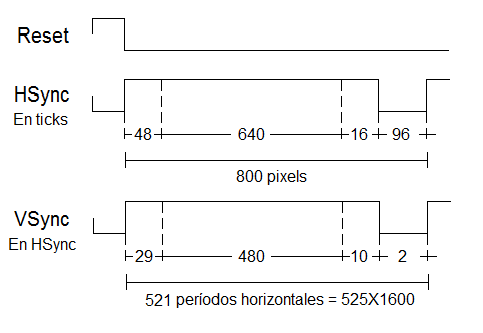
\includegraphics[width=10cm]{Img/DiagramaTiempos.png}
  \caption[3erNivel]{Diagrama de tiempos de contadores}
  \label{fig:DiagramaTiempos}
\end{figure}

No obstante, para seguir el diagrama del tercer nivel de la Figura \ref{fig:TercerNivel} y alimentar el contador horizontal con el reloj proporcionado de 100 MHz por parte de la Nexys 3 [2], se puede dimensionar el contador para que sea de 12 bits y ejecutar una división por 4, esto mediante el descarte de los dos primeros bits menos significativos. Por ello, el contador tendrá un tope de 3200 (800x4) y  serán aprovechados los primeros 10 bits más significativos. \\[2ex]
Por otra parte, el contador vertical debe incrementarse en cada ciclo del contador horizontal. En consecuencia, el contador vertical debe ser habilitado por el contador horizontal. De acuerdo con pruebas en el simulador, el contador interno horizontal (de 12 bits) debe levantar la bandera de conteo en los 1320 ticks, es decir, a la mitad del conteo para que haya un desfase correcto y los tiempos coincidan de forma correcta con errores despreciables. Esto permite que el generador de sincronía vertical inicie su pulso cuando el generador de sincronía horizontal finalice su pulso. Este contador tendrá un tope de 521, de acuerdo con lo visto en la Figura \ref{fig:DiagramaTiempos}.

\begin{figure}[htbp]
	\centering
	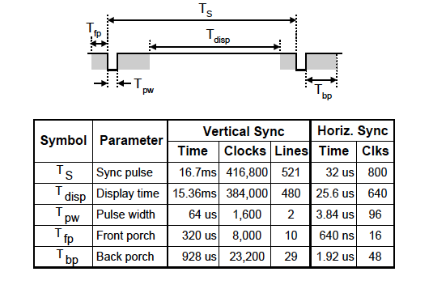
\includegraphics[ width=14cm]{Img/DiagramaTiemposExt.png}
	\caption[3erNivel]{Diagrama de tiempos de contadores}
	\label{fig:DiagramaTiemposExt}
\end{figure}

Los generadores de sincronía vertical y horizontal están diseñados de tal forma, que, cuando el contador horizontal tenga una magnitud de 0 a 96, se coloque un 0 en la salida \textquotedblleft H-Sync \textquotedblright y en caso contrario, la salida será 1. Algo similar ocurre con el contador vertical, que en este caso, la magnitud del contador vertical debe rondar los 0-2 para poder colocar un 0 en la salida \textquotedblleft V-Sync \textquotedblright.\\[2ex]
En cuanto al bloque de Memoria, este bloque es una memoria de acceso matricial, es decir, tiene doble direccionamiento. La primera forma de direccionamiento es la horizontal, que permite hacer una selección por filas. La segunda forma es la vertical, que permite seleccionar columnas. Esta memoria está dimensionada de 800 campos horizontales y 521 campos verticales. En total, se contabilizan 416800 espacios en la memoria. Asimismo, cada espacio cuenta con 2 bits, que permiten almacenar cuando se debe pintar una letra o fondo de pantalla o, bien, hacer un \textquotedblleft Blank \textquotedblright. Esta memoria, por tanto, permite establecer cuando debe hacerse la transmisión de los colores y cuando se deben apagar dichas señales en el \textquotedblleft Control de Salida \textquotedblright. Para entender la estructura de esta memoria, se propone la ilustración en la Figura \ref{fig:Memoria}\\[2ex]
Cabe destacar que, en el bloque de memoria, se han colocado las iniciales \textquotedblleft LLA \textquotedblright mediante los datos insertados y presentados en la Tabla \ref{tbl:Memoria}.\\[2ex]

\begin{figure}[htbp]
	\centering
	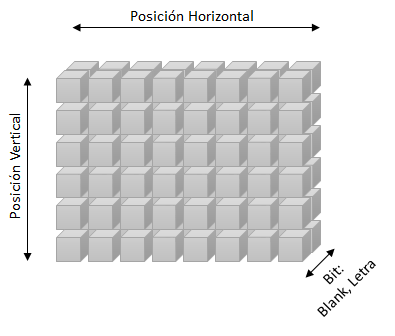
\includegraphics[ width=8cm]{Img/Memoria.png}
	\caption[3erNivel]{Estructura de la Memoria}
	\label{fig:Memoria}
\end{figure}

\begin{table}[]
	\centering
	\caption{Datos presentes en la Memoria para iniciales}
	\label{tbl:Memoria}
	
	\begin{tabular}{| c | c | c |}
		\hline 
		\textbf{Dato} & \textbf{Posiciones Horizontales} & \textbf{Posiciones Verticales}  \\
		\hline
		Blank = 1 y Letra = X & [0,48] U [688,800] & [0,30] U [510,521]  \\ [0.5ex] 
		\hline
		Blank = 0 y Letra = 1 & [0,48] U [688,800] & [0,30] U [510,521] \\ 
		\hline
	\end{tabular}
\end{table}

En general, el comportamiento de las etapas anteriores debe ser similar al presentado en la Figura \ref{fig:Comportamiento}. \\[2ex]
\begin{figure}[htbp]
	\centering
	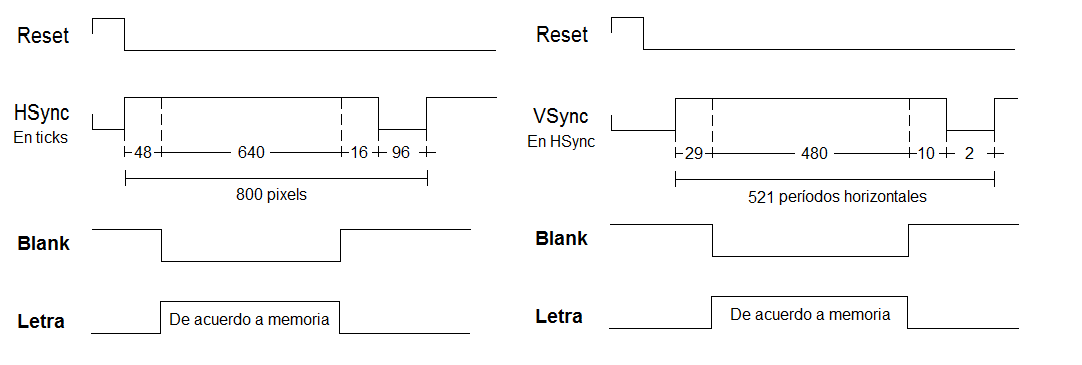
\includegraphics[ width=16cm]{Img/Comportamiento.png}
	\caption[3erNivel]{Estructura de la Memoria}
	\label{fig:Comportamiento}
\end{figure}

Asimismo, el \textquotedblleft Control de croma \textquotedblright, como su nombre alude, es donde se realiza el control de los colores y los tonos. Este control permite almacenar las configuraciones de forma volatil seleccionadas por el usuario mediante las entradas Up, Down, LP y TC (Tone). De esta forma, se transmite los colores que tendrán las letras y el fondo de pantalla, para que sea regulado mediante el \textquotedblleft Control de Salida \textquotedblright, al recibir las señales de Letra y de Blank. \\[2ex]
Por otro lado, el \textquotedblleft Control de Salida \textquotedblright permite modificar las salidas de los colores analógicos para modificar los tonos. Este control maneja las entradas digitales del DAC para poder hacer cambios en la tensión de la señales de R, G y B.\\[2ex]


\begin{figure}[htbp]
	\centering
	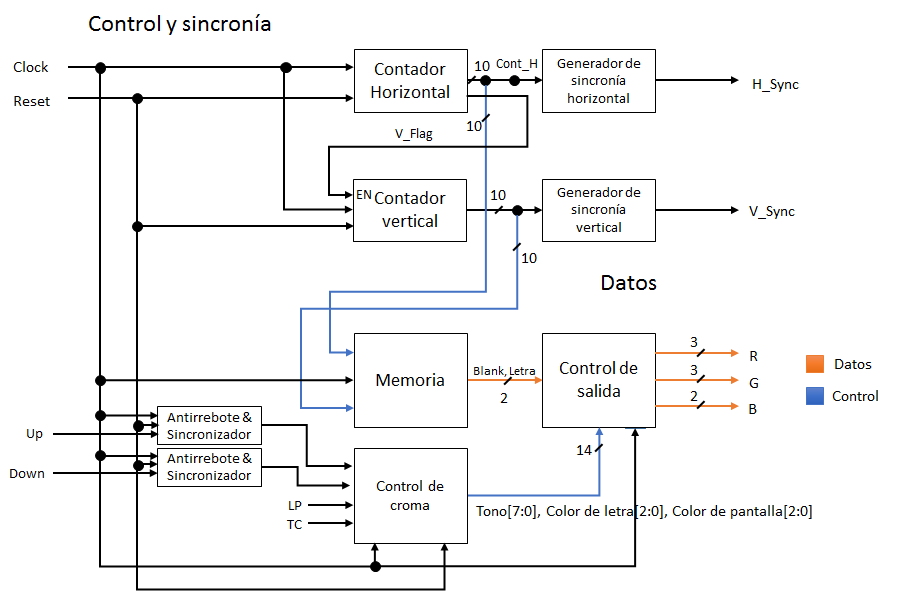
\includegraphics[ width=18.5cm]{Img/TercerNivel.png}
	\caption[3erNivel]{Interfaz del VGA.}
	\label{fig:TercerNivel}
\end{figure}

Finalmente, a continuación se presenta un resumen de las entradas y salidas de cada bloque, para aclarar las necesidades del diseño de tercer nivel. Véase la Tabla \ref{tbl:IO3}.

\begin{table}[]
	\centering
	\caption{Tabla de entradas y salidas del circuito}
	\label{tbl:IO3}
	\begin{tabular}{|l|l|l|}
		\hline
		\multicolumn{1}{|c|}{\textbf{Bloque}}                      & \textbf{Entradas / Salidas}                                          & \textbf{Ancho} \\ \hline
		\multicolumn{1}{|c|}{\multirow{4}{*}{Contador Horizontal}} & (Entrada) CLK: Corresponde al reloj del sistema.                     & 1              \\ \cline{2-3} 
		\multicolumn{1}{|c|}{}                                     & (Entrada) Reset: Permite reiniciar el contador                       & 1              \\ \cline{2-3} 
		\multicolumn{1}{|c|}{}                                     & (Salida) Cont\_H: Es el resultado del contador.                      & 10             \\ \cline{2-3} 
		\multicolumn{1}{|c|}{}                                     & (Salida) V\_Flag: Incrementa el contador vertical                    & 1              \\ \hline
		\multirow{3}{*}{Contador Vertical}                         & (Entrada) CLK: Corresponde al reloj del sistema                      & 1              \\ \cline{2-3} 
		& (Entrada) Reset: Permite reiniciar el contador                       & 1              \\ \cline{2-3} 
		& (Salida) Cont\_V: Es el resultado del contador.                      & 10             \\ \hline
		\multirow{2}{*}{Generador H-Sync}                          & (Entrada) Cont\_H: Es el resultado del contador H.                   & 10             \\ \cline{2-3} 
		& (Salida) H-Sync: Salida al monitor                                   & 1              \\ \hline
		\multirow{2}{*}{Generador V-Sync}                          & (Entrada) Cont\_V: Es el resultado del contador V.                   & 10             \\ \cline{2-3} 
		& (Salida) V-Sync: Salida al monitor                                   & 1              \\ \hline
		\multirow{4}{*}{Memoria}                                   & (Entrada) Cont\_H: Es el resultado del contador H                    & 10             \\ \cline{2-3} 
		& (Entrada) Cont\_V: Es el resultado del contador V.                   & 10             \\ \cline{2-3} 
		& (Salida) Blank: Alerta de señales de sincronía en Control de salida  & 1              \\ \cline{2-3} 
		& (Salida) Letra: Determina si se debe pintar una letra o fondo        & 1              \\ \hline
		\multirow{4}{*}{Antirrebotes \& Sinc.}                     & (Entrada) CLK: Corresponde al reloj del sistema                      & 1              \\ \cline{2-3} 
		& (Entrada) Reset: Permite reiniciar el contador                       & 1              \\ \cline{2-3} 
		& (Entrada) Botón: Recibe la señal del botón                           & 1              \\ \cline{2-3} 
		& (Salida) Bit: Salida libre de rebotes y sincronizada                 & 1              \\ \hline
		\multirow{9}{*}{Control de Croma}                          & (Entrada) CLK: Corresponde al reloj del sistema                      & 1              \\ \cline{2-3} 
		& (Entrada) Reset: Permite reiniciar el contador                       & 1              \\ \cline{2-3} 
		& (Entrada) Up: Permite incrementar un registro                        & 1              \\ \cline{2-3} 
		& (Entrada) Down: Permite decrementar un registro                      & 1              \\ \cline{2-3} 
		& (Entrada) TC: Modifica el tono del color                             & 1              \\ \cline{2-3} 
		& (Entrada) LP: Modifica el color de la pantalla o de la letra         & 1              \\ \cline{2-3} 
		& (Salida) Tono: Representa el tono seleccionado por el usuario        & 8              \\ \cline{2-3} 
		& (Salida) Color\_P: Contiene el color del fondo de pantalla           & 3              \\ \cline{2-3} 
		& (Salida) Color\_L: Contiene el color de la letra                     & 3              \\ \hline
		\multirow{9}{*}{Control de Salida}                         & (Entrada) CLK: Corresponde al reloj del sistema                      & 1              \\ \cline{2-3} 
		& (Entrada) Tono: Representa el tono seleccionado por el usuario       & 8              \\ \cline{2-3} 
		& (Entrada) Color\_P: Contiene el color del fondo de pantalla          & 3              \\ \cline{2-3} 
		& (Entrada) Color\_L: Contiene el color de la letra                    & 3              \\ \cline{2-3} 
		& (Entrada) Blank: Alerta de señales de sincronía en Control de salida & 1              \\ \cline{2-3} 
		& (Entrada) Letra: Determina si se debe pintar una letra o fondo       & 1              \\ \cline{2-3} 
		& (Salida) R: Representa la combinación de tonos de rojo al DAC        & 3              \\ \cline{2-3} 
		& (Salida) G: Representa la combinación de tonos de verde al DAC       & 3              \\ \cline{2-3} 
		& (Salida) B: Representa la combinación de azul de rojo al DAC         & 2              \\ \hline
	\end{tabular}
\end{table}

\section{Datos y resultados}
\subsection{Simulaciones}


\subsection{Mediciones}


\section{Análisis de datos y resultados}
En las simulaciones podemos notar que al realizar \textquotedblleft la simulacion postsintesis \textquotedblright estos tiempos se pueden considerar iguales a los del diagrama de tiempos de la figura \ref{fig:DiagramaTiempos}.\\[2ex]
Por otro lado, podemos notar que al usar un dispositivo de medición virtual, tales como el \textquotedblleft MyDaq \textquotedblright no se puede obtener una imagen precisa de la señal generada por las salidas, esto se debe a la alta frecuencia a la que oscila las salidas. Por lo que se debe usar instrumentos de medicion reales, un osciloscopio.\\[2ex]

\section{Hoja de datos de unidades desarrolladas}


\section{Conclusiones y recomendaciones}
\subsection{Conclusiones}
\begin{itemize}
    \item El desarrollo de la descripción de hardware a alto nivel, aprovechando el lenguaje Verilog y el sintetizador incorporado en Xilinx ISE facilita la tarea de implementación de un diseño para su futuro prototipado. Asimismo, el sintetizador permite aprovechar al máximo los recursos de una FPGA.
    \item El empleo de la simulación pre-síntesis permite monitorizar el comportamiento del código de una forma ideal y guía el desarrollo de la implentación por HDL.
    \item La simulación post-síntesis a nivel de compuertas es una gran herramienta para comprobar la compatibilidad de lo implementado en HDL para verificar su correcto funcionamiento al momento de transferirlo a una FPGA.
    \item El empleo de herramientas de control de versiones son una muy buena práctica para desarrollar código entre uno o varios programadores y para corrección de posibles errores.
    \item Es posible controlar un monitor mediante el protocolo VGA. Este protocolo es bastante flexible para poder desplegar datos, ya que facilita un control pixel por pixel en el monitor y eso puede flexibilizar la exposición de datos en la pantalla.
\end{itemize}

\subsection{Recomendaciones}
\begin{itemize}

    \item Durante la etapa de planificación y diseño, es necesario que todos los miembros del equipo estén presentes e involucrados, ya que esto permitirá mayor fluidez en el desarrollo del proyecto y el entendimiento del mismo.
    \item Es necesario, además, que los miembros del equipo tengan una buena comunicación y delimitar los roles que cada miembro tiene. Esto evitará futuros choques en las tareas de cada miembro.
    \item Se debe considerar, al inicio del trabajo, la plataforma de desarrollo que se empleará. Esto evitará modificaciones en el diseño en el momento de implementar el prototipo. Es bueno, también, tener a mano durante todo el diseño y la descripción en HDL, la hoja de datos de la plataforma.
    \item Crear un cronograma de trabajo sintetizado y asignar tareas por objetivos ayuda a tener una buena organización del equipo en cuanto al tiempo disponible para las tareas. Esto evitará contratiempos y posibles choques en las tareas.
    \item Se debe explorar con bastante anterioridad las herramientas de software que se emplearán durante el proyecto. Esto evitará posibles contratiempos al aprender a usarlas durante la implementación del proyecto.
    \item Simular de forma detallada un circuito permite encontrar posibles fuentes de error, tal como sirvió de ayuda para encontrar el desfase de las señales de sincronía de forma adecuada para que se cumplieran los tiempos de forma casi exacta a lo expresado por el fabricante.
    
\end{itemize}

\begin{thebibliography}{3}
\bibliographystyle{unsrtnat} % Use the "unsrtnat" BibTeX style for formatting the Bibliography

\bibitem[1]{PongChu}
Chu, Pong P. (2008)
\newblock \emph{FPGA prototyping by Verilog examples. Xilinx SpartanTM-3 Version},
\newblock John Wiley \& Sons, Inc.

\bibitem[2]{DatasheetNexys3}
Digilent. (2013)
\newblock \emph{Nexys3 Board Reference Manual},
\newblock Xilinx, Inc.

\end{thebibliography}

\end{document}
